\section{Evaluation}
\label{sec:eval}

In order to get an insight of the accuracy of the results generated by 
the implementation, the decision was made to test it against an 
application designed specifically for this purpose.

\subsubsection{High-level expectations}
\label{hw:eval:exp}

As outlined by \cite{pathak2012energy}, the power behaviour of the Wi-Fi 
mostly depends on the total network traffic and on the density of this 
traffic. If the antenna has to process some work-flow, it will remain in 
active mode and won't exhibit any tail-power behaviour. In this case, 
the traffic is really dense and the energy drain should be roughly 
proportional to the total traffic to process. However, one can imagine a 
situation where the antenna will have to process a small work-flow as 
soon as it enters its idle state. In this case, the traffic will be very 
sparse and the antenna will spend most of its time in tail mode. Based 
on these observations, the decision was made to build a test application 
which allows to generate traffic of various densities and to check 
whether the results generated by \Orka{} are fitting with these 
principles.

\subsubsection{Designing a test application}

An Android application was created using Android Studio to simply send a 
\texttt{HTTP GET} request every \texttt{T} milliseconds to a constant 
target URL. \texttt{T} was initially set to a thousand milliseconds and 
the target URL to \texttt{http://www.google.com}. After successfully 
monitoring the generated traffic using \Orka{}, a simple GUI was added 
to let the user specify the target URL and the parameter \texttt{T}.

\subsubsection{Running the tests}

\Orka{} was then run on this test application using the target URL 
\texttt{http://www.google.com} for various values of \texttt{T} between 
100ms and 4000ms in steps of 100ms. To this end, \monkeyrunner{} scripts 
were then generated in order to automatically set the right value of 
\texttt{T} and let \Orka{} monitor the traffic during 20 seconds. The 
results generated for $\texttt{T} = 1000ms$ are presented in Figure 
\ref{fig:tailfeedback}.

\subsubsection{Analysing the results}

At first glance, it was found that only the method 
\texttt{SendGet.run()}, which fires the \texttt{HTTP} request was 
attributed significant network usage, i.e.\ time in active and tail 
mode. All other methods were only attributed time in idle mode. This 
shows that \Orka{} was able to detect which method was producing network 
traffic, and therefore to map the hardware energy usage back to the 
code. Based on this, it is relevant to compare the energy-state tuples 
of the method \texttt{SendGet.run()} for all values of \texttt{T} and to 
check whether the expectations described in Section \ref{hw:eval:exp} 
were met. Figure \ref{fig:ggl:3:meth} shows the fraction of the time 
spent in each mode depending on the time \texttt{T} between each 
request.

\begin{figure}
  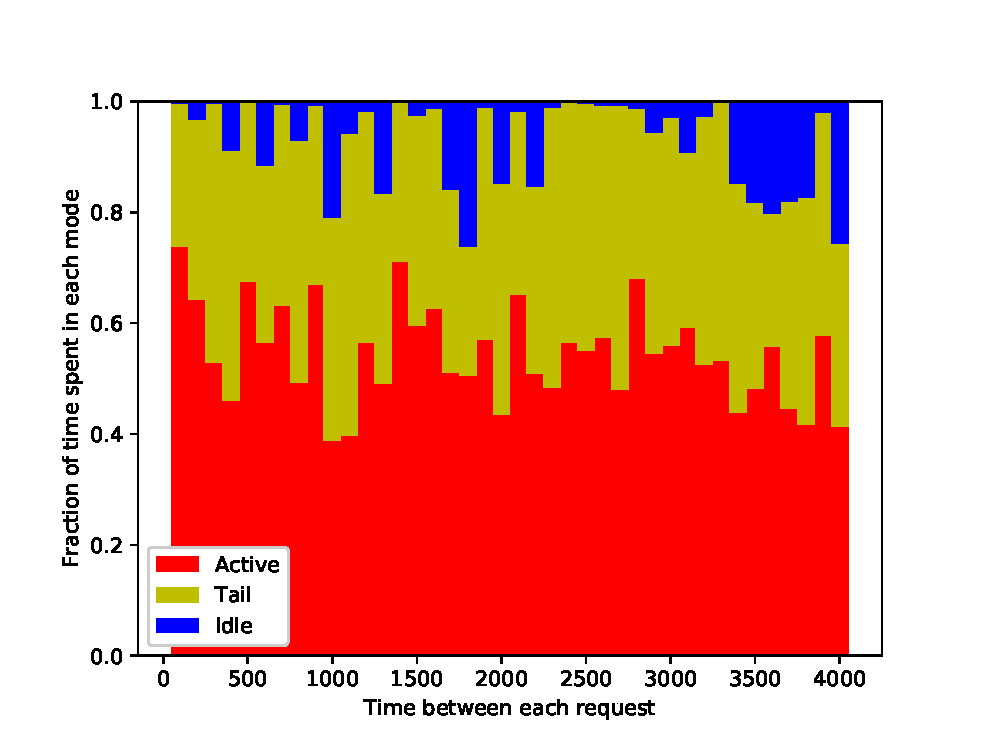
\includegraphics[width=0.5\textwidth]{figures/google_method_3states.eps}
  \caption{For the method \texttt{SendGet.run()}}
  \label{fig:ggl:3:meth}
\vspace {-0.32in}
\end{figure}

According to this graph, it seems that these ratios are constant with 
respect to the time between each request but include an important noise. 
This result may seem surprising at first, as the fraction of time spent 
in idle mode should increase with \texttt{T}, and as the fraction of 
time spent in tail mode should decrease with \texttt{T}. However, this 
result is explained by the fact that, to compute the energy tuple of a 
routine, the analyser only focusses on the Wi-Fi activity during the 
execution of this routine. Nevertheless, by definition, tail energy 
continues beyond the execution of the routine and \Orka{} is therefore 
failing to account for a part of the tail energy and of the time spent 
in idle mode. In order to improve the accuracy of the results at the 
method level, \Orka{} needs to implement more complex accounting 
policies, such as the last-trigger accounting policy, where the routine 
which last triggered a hardware component will be attributed the energy 
consumption that follows until another routine accesses this component.

To understand the Wi-Fi activity not attributed to any routine by 
\Orka{}, the decision was made to look at the energy tuples at the 
application level. The graph presented in Figure \ref{fig:ggl:3:glob} 
shows the fraction of the time spent in each mode depending on 
\texttt{T} at the application level. As expected, the fraction of time 
spent in idle mode increases as the traffic gets less dense but this 
graph doesn't allow us to draw conclusions about the active and tail 
modes, although it seems that the fractions of time spent in active and 
tail state are similar.

\begin{figure}
  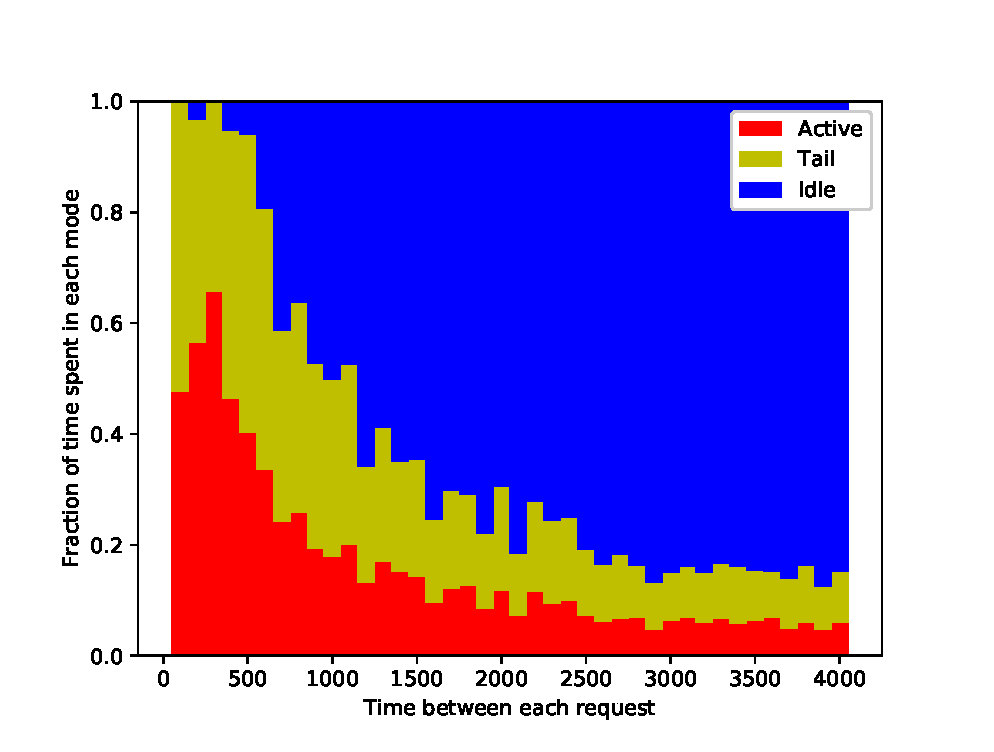
\includegraphics[width=0.5\textwidth]{figures/google_global_3states.eps}
  \caption{At the application level}
  \label{fig:ggl:3:glob}
\vspace {-0.32in}
\end{figure}


To focus on the active and tail modes, the two former graphs were 
regenerated taking only into account the time spent in these modes. At 
the method level, as the fraction of time spent in idle mode was small 
with respect to the fraction of time spent in the other modes, the graph 
focussing on the method \texttt{SendGet.run}, which is presented in 
Figure \ref{fig:ggl:2:meth}, is very similar to the one including the 
idle mode. The graph showing these results at the application level, 
which is presented in Figure \ref{fig:ggl:2:glob}, however shows that 
\orka{} attributes more time in tail mode as the traffic gets less dense 
and hence meets the high-level expectations described in Section 
\ref{hw:eval:exp}. Moreover, it seems that the fraction of the time 
spent in tail mode quickly reaches its maximum of about 60\%, for values 
of \texttt{T} higher than 500ms. Finally, according to these results, 
the Wi-Fi antenna spends at least 40\% of the time in tail mode, even 
for a dense traffic. This would suggest that at least 20\% of the drain 
caused by Wi-Fi is due to tail-behaviour.

\begin{figure}
  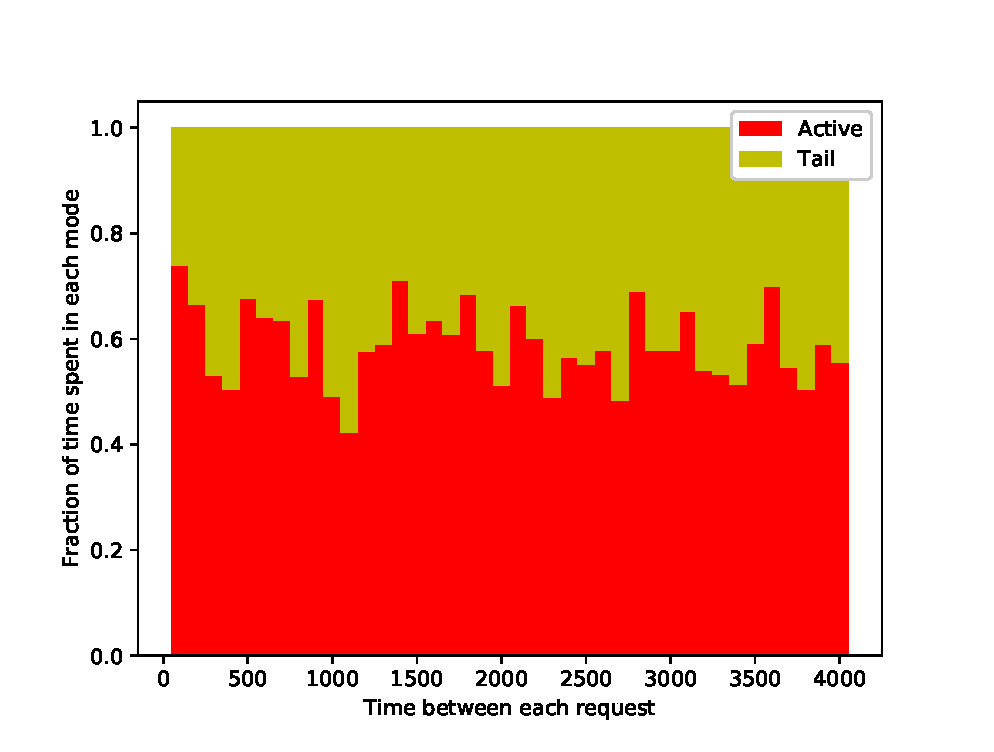
\includegraphics[width=0.5\textwidth]{figures/google_method_2states.eps}
  \caption{For \texttt{SendGet.run()}, ignoring idle mode}
  \label{fig:ggl:2:meth}
\vspace {-0.31in}
\end{figure}

\begin{figure}
  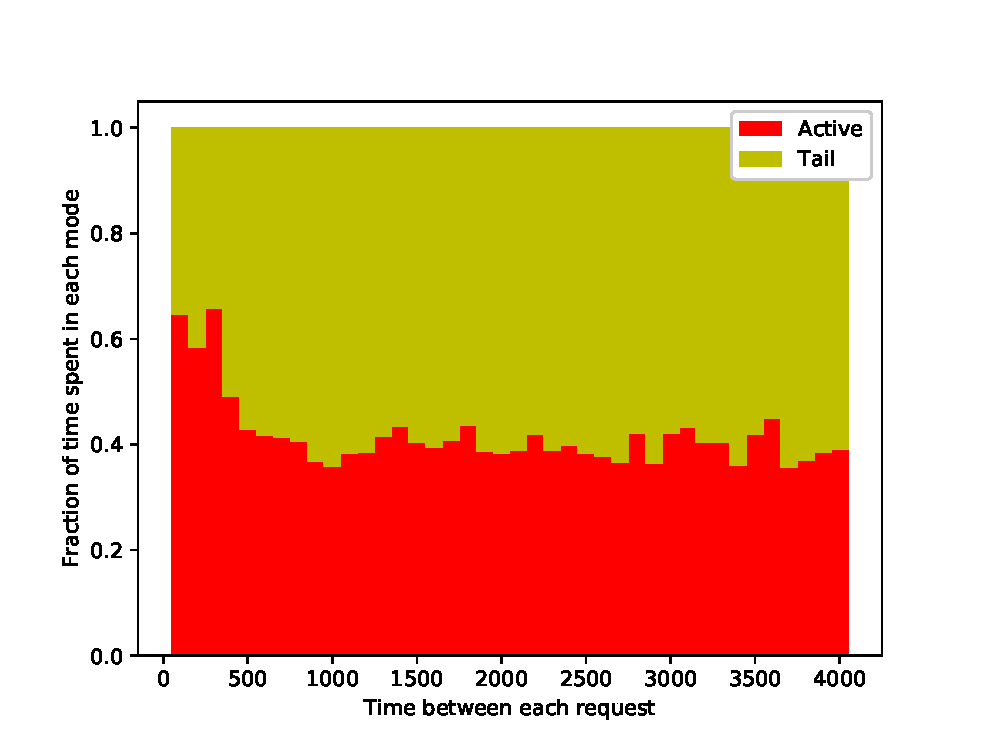
\includegraphics[width=0.5\textwidth]{figures/google_global_2states.eps}
  \caption{At the application level, ignoring idle mode}
  \label{fig:ggl:2:glob}
\vspace {-0.32in}
\end{figure}
